\section{Challenges and Problem Formulation}
\label{sec:problemformulation}

% Introduce the content of this section
In this section, we illustrate the challenges of hetergenous access point 
band selection in wireless network deployment and formulate the problem of band 
selection in mesh network deployments jointly using WiFi and white space bands. 
Further, we present a linear program and a FIXME algorithm for estimating the 
access point number to serve the traffic demand of a given population.
 
\subsection{White Space Opportunity and Challenge}
\label{subsec:motivation}

% Propagation
Wireless propagation is the behavior of the signal loss characteristics 
when wireless signals are transmitted through the wireless medium.
The strength of the received signal depends on both the line-of-sight
path (or lack thereof) and multiple other paths that result from 
reflection, diffraction, and scattering from 
obstacles~\cite{andersen1995propagation}. The widely-used Friis
equation characterizes the received signal power $P_r$ in terms 
of transmit power $P_t$, transmitter gain $G_t$, receiver gain $G_r$, 
wavelength $\lambda$ of the carrier frequency, 
distance $R$ from transmitter to receiver, and path loss exponent 
$n$ according to~\cite{friis}:
\begin{equation}
\label{eq:friis}
P_r=P_t+G_t+G_r+10n \log_{10}\left( \frac{\lambda}{4\pi R}\right)
\end{equation}
Here, $n$ varies according to the aforementioned environmental 
factors with the value of two to five in typical outdoor 
settings~\cite{rappaport}.

% Hetergenous access points
Despite sufficient levels of received signal, interference can cause channels
to be unusable (e.g., due to high levels of packet loss) or unavailable (e.g.,
due to primary users in cognitive radios~\cite{haykin2005cognitive}).
Prior work has worked to reduce cost through gateway deployment, channel 
assignment, and routing~\cite{he2008optimizing,tang2005interference}.
Most of existing works try to reduce the intra-network interference or increase
the channel usability level of wireless network deployment
~\cite{si2010overview,joshi2009efficient}. However, the access point service area
variation becomes an important problem when considering the availability of white space bands.  
Jointly considering the propagation and single channel capacity, the access points 
with different configuration (e.g. radios) in the same area, or with same configuration 
in diverse population density areas (e.g. downtown, rural) could have different service ranges.

% Explain multiband and hetergenous access points
When wireless devices operate in WiFi bands, the channel separation is relatively
small (e.g., 22 MHz for the 2.4 GHz band). As a result, many works assume that
the propagation characteristics across channels are similar. However, with the
large frequency gaps of WiFi and white space bands (e.g., several GHz),
propagation becomes a key factor in the deployment of wireless networks with both bands.
Here, a frequency band is defined as a group of channels which have
small separation meaning similar propagation characteristics.
In this work, we consider the diverse propagation and activity characteristics
for four total frequency bands: 450 MHz, 800 MHz, 2.4 GHz, and 5.2 GHz.
We refer to the two former frequency bands as white space bands and
the two latter frequency bands as WiFi bands.
A general way to increase the capacity of a single access point is to add channels
through radios~\cite{raniwala2005architecture}. The assumption all the channels have
the same propagation does not fit for WiFi and white space hetergenous scenario.
When a white space band channel added to an access point, the capacity and service 
range could increase simultaneously. The differences in propagation and constraints 
of network deployment create opportunity for the joint use of white space and 
WiFi bands in wireless access networks according to the environmental characteristics 
(e.g., urban or rural and downtown or residential) of the deployment location.

% Network Constraints
Typically, the deployment of wireless access networks is subject to coverage and capacity
constraints for a given region. Coverage is defined with respect to the ability of
clients to connect to access points within their service area.  We use a coverage
constraint ratio of $95\%$ in this work for a target area~\cite{robinson2010deploying}.
Capacity is defined with respect to the ability of a network to serve the traffic 
demand of clients.  Spatial reuse allows improved capacity, but increases the cost
of deploying a network by increasing the total number of access points required.
Hence, for densely populated areas the greatest level of spatial reuse possible
is often desired. And the deployment cost could be significant reduced through access 
points with high capacity with more centralized using radios. In contrast, 
sparsely-populated rural areas have lower traffic demand per unit area. Thus, 
aggregating this demand with lower-frequency, white space bands could be highly 
effective in reducing the total number of access points required to achieve 
similar coverage and capacity constraints. Moreover, since less TV channels tend
 to be occupied in sparsely populated areas~\cite{msdatabase}, a larger number 
 of white space bands can be leveraged in these areas. 




% Make multiband challenges
%The broadcast nature of the wireless induces interferences, 
%as both Inter-network and Intra-network interferences. 
%Avoiding the Intra-network interference has been deeply explored in 
%many works~\cite{subramanian2008minimum,ramachandran2006interference,si2010overview}.
%However, few of them try to address the inter-network interference.
%Due to the distribution nature of the Inter-network interference,
%it is difficult to build a theoretic model describing and estimating the activities of existing
%wireless signals. Measurement is the best and probably the only way 
% to tell the Inter-network interference. 



% Spectrum utility vary across different areas
%Jointly using WiFi and white space band adapting different 
%demands of rural area and urban areas is a key issue in 
%multiband wireless network deployment. 
%Thus, in sparsely-populated rural areas, the lower frequencies of the white space 
%bands might be a better choice for wireless service in sparsely populated areas. 
%However, as the population and demand scales up (e.g., 
%for urban regions), the greater levels of residents traffic demands 
%might detract the white space bands from the 
%overall deployment strategy. In such urban areas, select channels in 
%spacial reusable WiFi bands might be more appropriate, 
%since the degree of inter-network interference is often  
%proportional to the population (due to the existence of greater TV channels).

%The activity of inter-network interference is hard to tell in formula. 
%But from our measurements and TV station database, its activity correlate to the population distribution~\cite{msdatabase}.
%Figure~\ref{fig:drivemap} depicts a map of the available white space channels with
%markers where we performed measurements in North Texas. To be representative of a broad range of 
%community types, we consider populations of approximately 25 times one another according to the
%2010 U.S. Census, Millsap (500), Weatherford (25k), and Dallas (1.25 M). 
%
%%FIXME - put in experiment section
%As an initial experiment, 
%we perform a drive test from Dallas to Weatherford with cruise control set to 60 MPH while on
%the highway.  
%Part of the result of in-field spectrum measurement is shown in Figure~\ref{fig:drivetest}.
%The measured RSSI of 450 MHz is strong in downtown Dallas, downtown Fort Worth;
%but has less signal activity in the urban and rural area between these cities.
%The low activity level detected in WiFi bands is due to the distance from highway is larger
%than the propagation range of an indoor wireless router whose transmitting power is limited.
%The map itself shows the available white space channels in DFW area, more green means
%more channels. Our in-field measurement matches the FCC restriction showing that less channels means
%more spectrum utility and tell the spectrum utility levels varying across population 
%distribution. We also collect measurements at more fixed locations as marked on the map to collect
%data for the spectrum utility calculation. 
%\begin{figure}
%%\vspace{-0.0in}
%\centering
%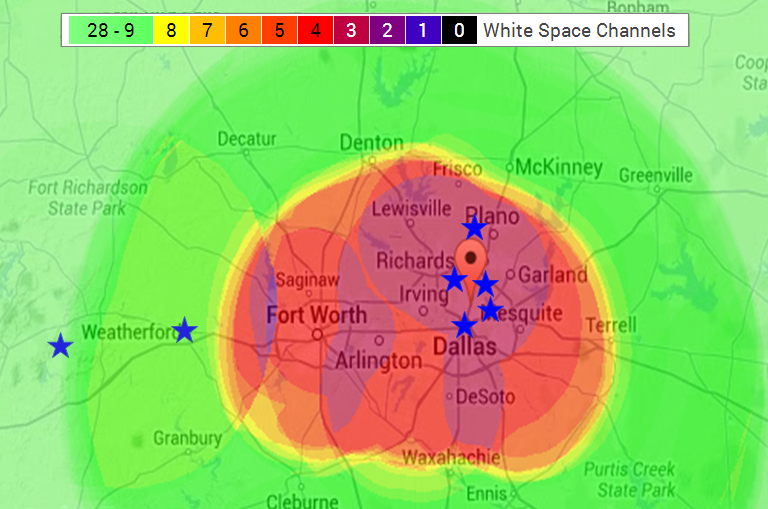
\includegraphics[width=74mm]{figures/drivemap}
%\vspace{-0.1in}
%\caption{DFW Metropolitan Measurement Location}                                                                 
%\label{fig:drivemap}
%\vspace{-0.1in}
%\end{figure}
%   
%\begin{figure}
%%\vspace{-0.0in}
%\centering
%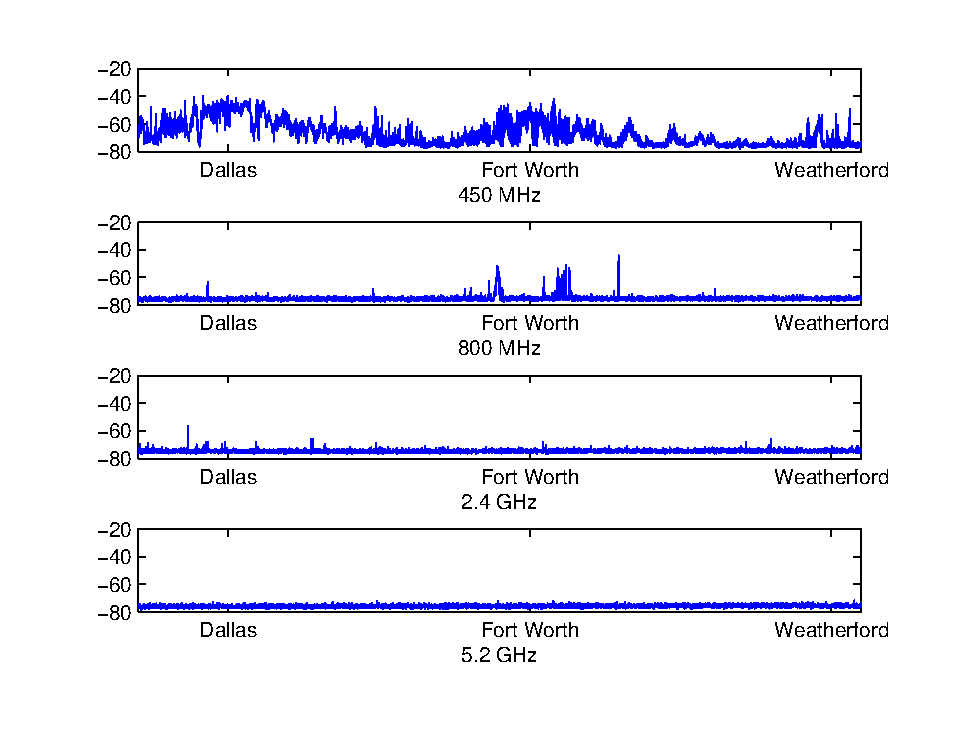
\includegraphics[width=94mm]{figures/drivetest}
%\vspace{-0.1in}
%\caption{Spectrum Activity In DFW}                                                                 
%\label{fig:drivetest}
%\vspace{-0.1in}
%\end{figure}
%
%% Fix location example claiming the activity is kind of stable
%Figure~\ref{fig:labact} depicts an example spectrum utility in activity level
%defined in~\ref{subsec:problem} in our urban lab with the platform introduced 
%in~\ref{sec:experimentdesign}. 
%The activity level from data collected in the same location shows 
%the difference in time domain. On average, the existing signals occupy 25.83 
%percentage of time in 450 MHz, 26.49 percentage of time in 800 MHz, 
%34.95 percentage of time in 2.4 GHz and 35.46 percentage of time in 5.2 GHz. 
%Our experiments show that in a fixed location, the spectrum utility is around
%a certain number in time domain. This character provides a method to tell
%the spectrum utility through measurements. These Inter-network interference 
%of existing signals have to be counted in wireless network deployment. 
%
%   \begin{figure}
%   %\vspace{-0.0in}
%   \centering
%   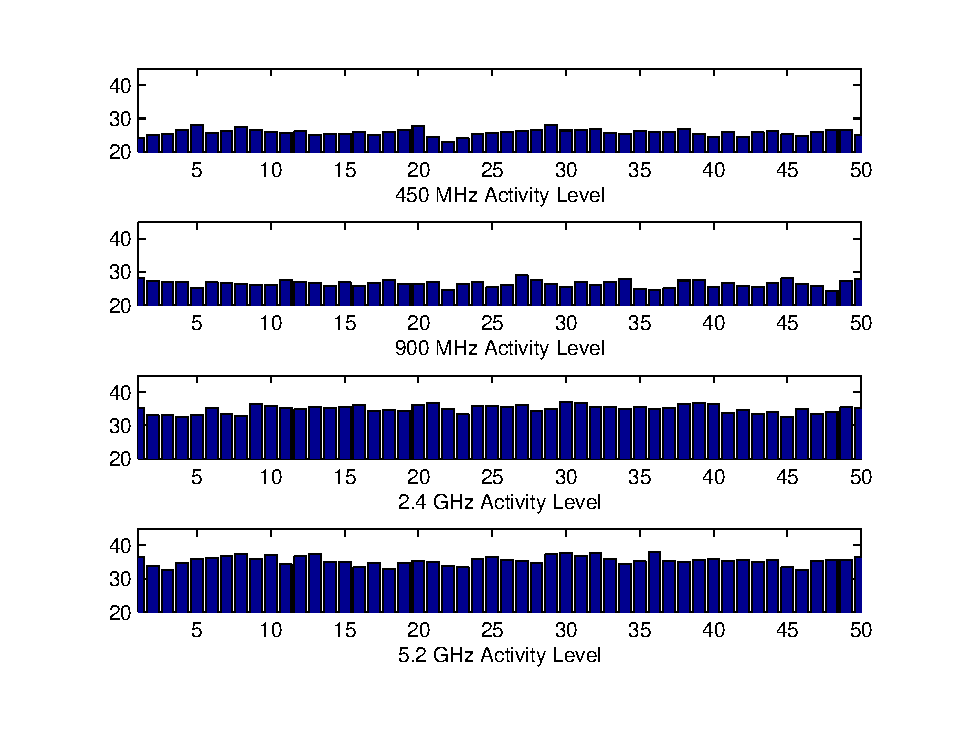
\includegraphics[width=94mm]{figures/labactivity}
%   \vspace{-0.1in}
%   \caption{Wireless Activity in Urban Lab}                                                                 
%   \label{fig:labact}
%   \vspace{-0.1in}
%   \end{figure}
%   
%In the measurements, there is around $10\%$ difference from white space 
%band to WiFi bands in our urban lab. This spectrum utility gap and multiband
%propagation variation in band selection of wireless network 
%deployment is what we have to notice. 
%

\subsection{Model and Problem Formulation}
\label{subsec:problem}

teasg
Here test
adgfasdfag



% Assumptions of the network
As opposed to previous works such as~\cite{tang2005interference,yuan2006cross
,si2010overview}, this paper focuses on reducing the inter-network
interference for various population densities for wireless access networks which
jointly employ WiFi and white space bands. We propose a measurement-driven 
framework to estimate the number of access points required for serving the traffic
demand of a certain area. We assume an access point has a limited number of radios
which operate on any channel of a fixed number of channels with the same antenna gain.
Each radio on an access point operates with a classic protocol model~\cite{gupta2000capacity}. 
We further assume that there is a given take rate and traffic demand for a given 
population (as specified in Section~\ref{sec:experimentdesign}).  
%Generally, Internet data request comes with population and Finland government even announce 
%broadband is an individual 'legal right'~\cite{bbcfinland,rosston2011household}. 
%Providing a community wireless Internet service have to satisfy its traffic demand 
%of the people in the area. 
%In populated urban areas, more people need more 
%network capacity in which case WiFi band spatial reuse is better than white space bands
%who limit the capacity in a large area. Moreover, in populated urban area, 
%more Inter-network interference comes from TV station and other sources in white space
%bands could reduce the capacity of a channel. However, in rural area, too many access points
%in WiFi bands for the large area is a waste of funding. Here we are trying to answer the question
% in a certain Inter-network interference, what is the band or bands combination we should 
% use to provide network service for a community with different population density.
%Since mathematical formula is difficult to describe the activities of 
%signal on the air even in an arbitrary area.

<<<<<<< HEAD

=======
>>>>>>> eb489c516f494a214506030432cf665bea1ffa4c
For spectrum utility and resulting channel availability, we use a long-term measurement 
for each band.  We define the percentage of sensing samples $S_\theta$ above an 
interference threshold $\theta$ over the total samples $S$ in a time unit as the 
activity level $A$ of inter-network interference:
\begin{equation}
\label{eq:actdef}
A=\frac{S_\theta}{S_a}
\end{equation}
The capacity of a clean channel is denoted by $C$. With the protocol model, the capacity 
of a channel with inter-network interference $C_r$ could be represented as 
the remaining time of the clean channel capacity according to: 
\begin{equation}
\label{eq:intercap}
C_r=C*(1-\bar{A})
\end{equation}

A network deployment should ideally provide network capacity equal to the demand of the service 
area to maintain the capacity constraint. The demand of a service area could be calculated as the 
summation of individual demands all over the service area $D_a=\sum_{p\in P}D_p$. Since 
household demand for Internet has been previously characterized~\cite{rosston2011household}, 
$D_a$ could represent the population distribution $f$ and service area $k$ as 
$D_a=\sum_{f \in F,k \in K}\bar{D_p}*f*k$. 
The capacity constraint could be represented with access points set $M$ according to:
\begin{equation}
\label{eq:nlbound}
\sum_{m \in M}C_r^m \ge \sum_{f \in F,k \in K}\bar{D_p}*f*k
\end{equation}
At the same time, the wireless network must additionally satisfy the coverage constraint in the service 
area where the access points provide connectivity for client devices. 
Generally, a coverage of $95\%$ is acceptable for wireless access networks~\cite{robinson2010deploying}.

In a joint white space and WiFi scenario, the activity level varies according to various interfering 
sources and the propagation characteristics induced by the environmental characteristics of the service area.
A simple method with the least number of access point to cover an area is to use 
multiple orthogonal lower-frequency channels. However, the FCC limits the white space band availability 
for data communication in most metropolitan areas in the United States~\cite{googledatabase}. Moreover, the 
number of channels in each band is limited. Too many lower-frequency channels will cause high levels of 
intra-network interference for the network, which is out of our scope in this work. We assume that the 
cost of the network is proportional to the number of access points required for a given user demand (i.e., due
to the cost of hardware and installation). Therefore, given a geographical region for a new network deployment
we build a measurement-driven framework called Multiband Access Point Estimation (MAPE) to compute the required
number of access points.

\begin{algorithm}[t]
\small
\caption{Multiband Access Point Estimation (MAPE)}
\label{algorithm:mape}
\begin{algorithmic}[1]
\REQUIRE  ~~\\
$A$: Measured Activity Level \\
$F$: Population Distribution\\
$C$: Clean Channel Capacity\\
$n$: Path Loss Exponent \\
$B$: Available frequency bands\\
$M$: Area need to be covered
\STATE Split $M$ in to different type, calculate the traffic demand density $f$
\STATE Calculate in-field channel capacity $C_r$ as $C(1-A)$
\STATE Get the propagation coverage area radius $R_p$ from Frii model based on $n,B,F$
\STATE Calculate the QoS coverage radius $R_{QoS}$ of a Multiband Access Point satisfy the demands of the area
\STATE The coverage radius of a Multiband Access Point is $Min{R_p,R_{QoS}}$
\STATE Apply regular hexagon deployment to get the number of access point for serving given area $M$
\ENSURE ~~\\
The number of Access Points\\
\end{algorithmic}
\end{algorithm}

% Fix the framework , Mark should use them in a single tower with more radios
% Framework
In the space domain, the advantage of higher-frequency channels is the spatial reuse, while
the lower-frequency channels provide greater levels of coverage. Generally, higher 
frequencies are more appropriate for populated areas, and lower frequencies are
more appropriate for sparse areas. The time-domain variation of spectrum utilization 
differs across bands.
%could be seen in Figure~\ref{fig:labact}.
For an internet service provider, the service quality which maps to the capacity constraint must be satisfied.
Given a metropolitan area, the population distribution can be found according to
government statistics~\cite{uscensus}. Then, we can estimate the capacity demand
of each type of area with the assumption that users will exhibit average demand.
According to the population distribution, we split the area into different types,
which compose the space-domain input. Then, we use the measured activity level as 
the time-domain input. We have an average channel capacity of each band according to the 
activity level. With the received signal strength threshold, the Quality-of-Service-constrained
coverage area of different types per channel, and the spatial reuse distance be directly
computed. Then, the maximum area an access point could cover can be calculated as the minimal
area of the QoS-based coverage area and propagation coverage.
Then, the transmit power is adjusted to fulfill the coverage restriction subject to
the FCC regulations for maximum-allowable transmit power. 
A classic regular hexagon deployment process is employed to place the access points.

%With this framework, we combine our measurements to evaluate white
%space bands application varying with population density in section~\ref{sec:experimentdesign}.



